\chapter{Vaatimustenkeruusuunnitelma} % Itse luvun otsikko. Huom ei numeroa!
\label{keruu} % Tähän kappaleeseen voi viitata \ref{keruu}
\thispagestyle{fancy} % Tarvitaan, jotta header/footer näkyvät otsikkosivuilla

Tässä luvussa käsitellään jo olemassa olevia dokumentaatioita, ja mitä vaatimuksia asiakastietojärjestelmälle voidaan niiden perusteella määrittää. Luvussa esitellään erilaisia tapoja, joita voidaan hyödyntää vaatimusten keruussa sidosryhmiltä.

\section{Taustatilanne}

% TODO pitäisiköhän tähän vielä lisätä jotain?
Megantti konsernilla ei ennestään ollut käytössä keskitettyä asiakkuudenhallintajärjestelmää (\acrshort{crm}).
Asiakastietoja ovat keränneet lähinnä myyntipuolen työntekijät, joilla on ollut ongelmia tietojen jakamisessa keskenään sekä asiakastietojen tietosuojaan liittyen. Uuden CRM:n olisi tarkoitus keskittää tietojen hallinnointi ja tasapuolistaa erityisesti eri myyntihenkilöiden informatiivista asemaa asiakkaita kohtaan.

\section{Nykyisen dokumentaation analyysi}

% TODO Kaksi otsikkoa peräjälkeen.. Tähän 2 lasuetta?

    \subsection{Kehyskertomuksen analyysi}
    Con-Salting Oy on kerännyt alustavia vaatimuksia kehyskertomukseen. Kehyskertomuksessa määritetään asiakastietojärjestelmälle alustavia vaatimuksia. Kehyskertomuksen perusteella voidaan määrittää sidosryhmiä, jotka tulee ottaa huomioon, ja joiden kanssa tulee kommunikoida vaatimuksia määriteltäessä.

    Tällaisia sidosryhmiä ovat muun muassa yrityksen johto ja myynti- ja markkinointiosasto.
    sidosryhmät ovat esittäneet toivomuksina esimerkiksi asiakastietojärjestelmän nopean toiminnan, käytettävyyden erilaisilta päätelaitteilta sekä asiakkaan 
    automaattisen profiloinnin. 
        
    Kehyskertomuksessa ilmenee myös muita asioita jotka tulee ottaa huomioon:
    
    \begin{itemize}
        \item Järjestelmän tulee olla yhteensopiva muiden yrityksen järjestelmien kanssa kuten yrityksen varastojärjestelmän kanssa.
	\item Asiakastietojärjestelmän tulee myös olla \gls{gdpr} mukainen
        \item Järjestelmän tulee pystyä hoitamaan joitain asioita automaattisesti, kuten suurostobonukset.
    \end{itemize}

    Nämä vaatimukset ovat kuitenkin ainoastaan suuntaan antavia, ja niitä tulee tarkentaa vaatimustenkeruussa. 


\section{Vaatimustenkeruumetodit}

    Vaatimustenkartutusmetodit voidaan jakaa kahteen eri osa-alueeseen: Epäsuoriin- ja suoriin metodeihin.
    Tässä kappaleessa käsitellään Megantin asiakastietojärjestelmän kehitystä varten käytettäviä metodeja.


    \section*{Suorat metodit}

        Suorissa kartutustekniikoissa järjestelmän vaatimuksia kartoitetaan yhdessä sidosryhmien kansssa.
        Käytämme seuraavia suorakartutustekniikoita:

        \subsubsection*{Haastattelut}

            Järjestämme kahdentyyppisiä haastatteluja sidosryhmille. Toisessa haastattelussa haastateltavat vastaavaat ennaltamääriteltyihin kysymyksiin. 
            Toisessa haastattelussa haastattelu toteutetaan avoimesti. Haastateltaville esitetään erilaisia kysymyksiä järjestelmän toiminnalisuuteen liittyen jolloin
            haastateltavien kanssa voidaan vuorovaikutteisesti pohtia millainen järjestelmän tulisi olla.

        \subsubsection*{Havainnointi}

            Lähetämme 2 kehitystiimiläistä vierailemaan  Meganttiin. Nämä tiimiläiset seuraavat päivän ajan Megantin työntekijöiden työtä, ja tekevät 
            muistiinpanoja työntekijöiden tarpeista järjestelmään liittyen. He havainnoivat myös mitä puutteita ja vahvuuksia nykyisessä asiakastietojärjestelmässä on.
            Käytämme havainnointia siitä syystä, että ihmisten on usein vaikea pukea arkipäivän työntekoa sanoiksi. Havainnoin avulla pääsemme eroon tästä haittatekijästä.


        \subsubsection*{Ryhmätapaamiset}

            Projektin aikana järjestetään tapaamisia sidosryhmien kanssa. Näissä tapaamisissa kehitystiimi kertovat asiakastietojärjestelmän nykytilasta, kuvailevat tilanteita 
            johon sidosryhmät voivat vastata kuinka he haluavat järjestelmän toimivan kyseisissä tilanteissa.


    \section*{Epäsuorat metodit}

        Epäsuorissa kartutustekniikoissa sidosryhmiin ei olla suorassa kontaktissa, vaan käytetään jo ennalta olevia tietoja.
        Käytämme seuraavia epäsuorakartutustekniikoita:

        \subsubsection*{Taustatutkimus}

        Con-Salting Oy on kerännyt jo muutamia yrityksen vaatimuksia kehyskertomukseen. 
        Näitä vaatimuksia ovat esimerkiksi asiakastietojen ylläpito, ja asiakkaiden profilointi.
        Vaatimukset ovat kuitenkin löysästi määriteltyjä ja vaativat tarkennusta.

        \subsubsection{Kyselyt}

        Osalle järjestelmän sidosryhmistä järjestetään kyselyitä, jossa selvitetään heidän mielestään tärkeimpiä järjestelmän vaatimuksia.
        Tällaisia sidosryhmiä ovat sisäiset käyttäjät, kuten yrityksen johto, asiakaspalvelu ja järjestelmän ylläpito henkilöstö.

        \subsubsection*{Prototyypit}

        Sisäisille käyttäjille valmistetaan kahteen otteeseen prototyyppi järjestelmästä. Käyttäjät voivat siis testata järjestelmää aikaisessa vaiheessa ja antaa palautetta.
\section{Sidosryhmäanalyysi}

    \subsection{Iso kuva}

        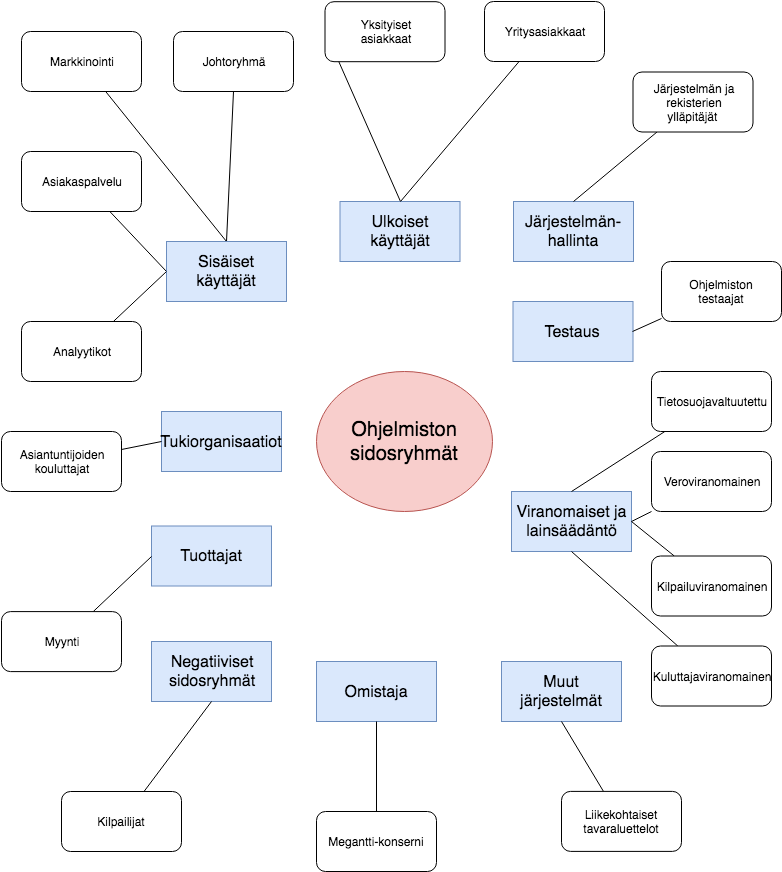
\includegraphics[width=\textwidth]{sidosryhmat.png}
        \label{img:sidosryhmat.png}